%==============================================================================
\section{System Model}
\label{sec:model}
%==============================================================================

\subsection{Normalized Aggregation With Private Weights}

An FC and $N$ single-antenna devices cooperate to compute, for each \emph{aggregation instance},
\begin{equation}
\vo=\frac{\vn_A+\sum_{j=1}^N d_j\obar_j}{d_A+\sum_{j=1}^N d_j}\in\R^{d_v},
\label{eq:target}
\end{equation}
where $(d_A,\vn_A)$ is an anchor term held by the FC, $d_j\ge0$ is the weight of device $j$ and $\obar_j$ its local normalized output, with $\|\obar_j\|\le V_{\max}$. The weights are \emph{private}: $d_j$ is computed at device $j$ from information broadcast by the FC and from data that only device $j$ holds, and the FC does not know $\{d_j\}$ before or after the aggregation. We write $D=\sum_j d_j$ for the device mass and
\begin{equation}
\Neff=\frac{\big(\sum_j d_j\big)^2}{\sum_j d_j^2}\in[1,N]
\label{eq:neff}
\end{equation}
for the participation ratio of the weights: $\Neff=N$ when the mass is spread evenly and $\Neff\approx1$ when one device dominates.

\emph{Sharded-KV attention.} Consider decoding with a KV cache whose context is split into $N$ contiguous shards $\mathcal{S}_j$, one per device. For a query $\vq$ of one head in one layer, device $j$ computes the logits $s_i=\vq^{\mathsf T}\vk_i/\sqrt{d_k}$ of its tokens and returns $d_j=\sum_{i\in\mathcal{S}_j}e^{s_i-c}$ and $\vn_j=d_j\obar_j=\sum_{i\in\mathcal{S}_j}e^{s_i-c}\vv_i$. The FC holds an anchor block (the first tokens, which contain the system prompt and the attention sink~\cite{xiao2024streaming}) and the tail from the question on, including the generated tokens, in the spirit of the anchor block of~\cite{acharya2025star}. It sets $c$ to the maximum of its own logits, so no extra round is needed to agree on the shift, and $(d_A,\vn_A)$ collects its own terms. Then~\eqref{eq:target} is exactly the attention output. Since $\obar_j$ is a convex combination of value vectors, $V_{\max}$ can be taken as the largest value norm of the head, calibrated offline. Fig.~\ref{fig:system} sketches the system and the protocol of Section~\ref{sec:design}.

\begin{figure}[t]
\centering
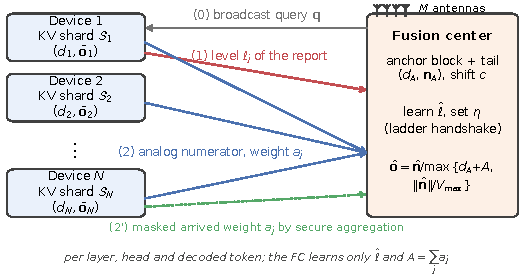
\includegraphics[width=\linewidth]{fig_system.pdf}
\caption{Sharded-KV decoding over the air. Per layer, head and decoded token, the FC broadcasts the query (0); the devices announce the level of their noise-matched report through a digital or tone handshake (1) and transmit their scaled partial outputs, which superpose at the $M$-antenna FC (2); the weights with which they arrive are securely aggregated in parallel (2').}
\label{fig:system}
\end{figure}

\emph{Spatial regression.} In Nadaraya--Watson regression with a Gaussian kernel, $d_j=\exp(-\|\mathbf{x}_\star-\mathbf{x}_j\|^2/2h^2)$ and $\obar_j=y_j$ for a sensor at $\mathbf{x}_j$ with measurement $y_j$ and a query location $\mathbf{x}_\star$; this is softmax attention with distance logits. The FC may add a prior pseudo-observation $(d_A,\vn_A)=(w_0,\mathbf{0})$. In product-of-experts Gaussian-process regression~\cite{sato2022gpr}, $d_j=\sigma_j^{-2}(\mathbf{x}_\star)$ and $\obar_j=\mu_j(\mathbf{x}_\star)$ are the local posterior precision and mean of expert $j$.

\subsection{Channel and Receiver}

The FC has $M$ antennas. The channel of device $j$ is $\vh_j=\sqrt{\beta_j}\,\tilde{\vh}_j\in\C^M$, where $\beta_j$ is the large-scale gain and $\tilde{\vh}_j\sim\mathcal{CN}(\mathbf{0},\mathbf{I}_M)$; the channels are independent across devices and constant over one instance. The FC applies a unit-norm receive combiner $\vm$ chosen from the channels only---it cannot use the weights---and device $j$ sees the effective gain
\begin{equation}
g_j=|\vm^{\mathsf H}\vh_j|^2 .
\end{equation}
For $M=1$, $g_j=\beta_j|\tilde h_j|^2$ is exponential with mean $\beta_j$. In the analysis we also allow Nakagami-$m$ fading, $|\tilde h_j|^2\sim\mathrm{Gamma}(m,1/m)$. Each device knows its effective channel $\vm^{\mathsf H}\vh_j$, which it can estimate from a downlink pilot precoded with $\vm$ under channel reciprocity.

\subsection{Transmission and Estimator}

We adopt the convention of~\cite{yang2026airmoe}: the weight is placed in the precoder and the data are normalized. Device $j$ transmits $d_v+1$ real streams, the denominator stream with datum $1$ and the numerator streams with data $\obar_j/\sigma_o$, where $\sigma_o$ is an offline root-mean-square value of the outputs, all with the same precoder
\begin{equation}
b_j=\frac{\eta\,d_j}{\sqrt{g_j}}\,e^{-\jmath\angle(\vm^{\mathsf H}\vh_j)},\qquad |b_j|^2\le P .
\label{eq:precoder}
\end{equation}
Here $\eta>0$ is a scale common to all devices. A device for which $\eta^2d_j^2/g_j>P$ cannot invert its channel and transmits at full power; its weight then arrives attenuated as $a_j=\sqrt{Pg_j}/\eta<d_j$. In general $a_j=\min\{d_j,\sqrt{Pg_j}/\eta\}$. After combining, phase compensation and normalization by $\eta$, the FC observes
\begin{align}
\hat D&=d_A+\sum_j a_j+\frac{z_0}{\eta}, \label{eq:Dhat}\\
\hat\vn&=\vn_A+\sum_j a_j\obar_j+\frac{\sigma_o}{\eta}\vz, \label{eq:Nhat}
\end{align}
with $z_0\sim\mathcal{N}(0,1)$ and $\vz\sim\mathcal{N}(\mathbf{0},\mathbf{I}_{d_v})$, i.e., real noise of unit variance per stream; the signal-to-noise ratio is $\snr=P$. The FC outputs
\begin{equation}
\hat\vo=\frac{\hat\vn}{\max\{\hat D,\ d_A,\ \|\hat\vn\|/V_{\max}\}},
\label{eq:estimator}
\end{equation}
where the floor is the convex-hull projection of Section~\ref{sec:design}; we call~\eqref{eq:estimator} the \emph{analog ratio}. One instance occupies $d_v+1$ real channel uses whatever $N$ is; an LLM layer with $H$ query heads needs $H(d_v+1)$ real symbols per decoded token.

The design problem is the choice of the scalar $\eta$ for every instance. If the FC knew the weights, the largest scale that avoids saturation would be the \emph{genie} scale
\begin{equation}
\eta_{\rm g}^2=\frac{P}{B},\qquad B=\max_j\frac{d_j^2}{g_j},
\label{eq:genie}
\end{equation}
so that the effective noise variance on $\hat D$ is $B/P$. We call $B$ the \emph{mass-weighted bottleneck}; it couples the private weights with the channels, and it is the central random variable of Section~\ref{sec:analysis}.

\subsection{Information Structures}

Different ways of conveying the denominator and the scale reveal different information to the FC. Table~\ref{tab:schemes} lists the schemes compared in this paper. Blind analog aggregation reveals only the noisy sums but, as shown in Section~\ref{sec:analysis}, it pays a large penalty when the weights are dispersed. The designs of Section~\ref{sec:design} add an anonymous handshake per instance, which in its digital form reveals at most the highest occupied level of a ladder. The analog ladder keeps the over-the-air denominator $\hat D$; the non-saturating split ratio replaces it by the exact sum $D$ obtained by secure aggregation; the proposed design replaces it by the sum $A=\sum_ja_j$ of the weights that arrive. A secure digital merge reveals only the exact sums but must securely aggregate all partials. Known-weight aggregation~\cite{yang2026airmoe} and orthogonal access reveal every device's weight, and the latter also every device's output.

\begin{table}[t]
\centering
\caption{Schemes and what the FC learns per instance. Rounds: uplink rounds per layer after the query broadcast; digital uplink: scalars per layer ($^\ast$plus $NHL$ bytes with the digital handshake); $\hat\ell$: handshake information (Proposition~\ref{prop:leakage}).}
\label{tab:schemes}
\setlength{\tabcolsep}{3pt}
\begin{tabular}{@{}lccl@{}}
\toprule
Scheme & Rounds & Digital uplink & FC learns \\
\midrule
Blind (fixed $\eta$) & 1 & -- & $\hat\vn,\hat D$ \\
Analog ladder & 2 & -- & $\hat\vn,\hat D,\hat\ell$ \\
Non-saturating split & 2 & $NH$ masked$^\ast$ & $\hat\vn,D,\hat\ell$ \\
Proposed & 2 & $NH$ masked$^\ast$ & $\hat\vn,A,\hat\ell$ \\
Secure digital merge & 1--2 & $NH(d_v+1)$ masked & $\vn,D$ \\
Known weights~\cite{yang2026airmoe} & 2 & $NH$ & $\hat\vn$, all $d_j$ \\
ZF-TDMA & 1 & $NH$ & all $\obar_j$, $d_j$ \\
Digital LSE merge & 1 & $NH(d_v+1)$ & all $\obar_j$, $d_j$ \\
\bottomrule
\end{tabular}
\end{table}

\subsection{Performance Metrics}

For a single instance we use the outage of the denominator and the saturation probability. End to end, for LLM decoding we measure the Kullback--Leibler divergence $\mathrm{KL}(p_{\rm ref}\|p_{\rm air})$ between next-token distributions, the increase of the next-token negative log-likelihood (NLL), the top-1 agreement, and needle-in-a-haystack (NIAH) retrieval accuracy, all against the exact shard merge as reference. For spatial regression we use the root-mean-square error (RMSE) over the query points of a round.
